\documentclass[a4paper]{article}

%% Language and font encodings
\usepackage[english]{babel}
\usepackage[utf8x]{inputenc}
\usepackage[T1]{fontenc}

%% Sets page size and margins
\usepackage[a4paper,top=3cm,bottom=2cm,left=3cm,right=3cm,marginparwidth=1.75cm]{geometry}

%% Useful packages
\usepackage{amsmath}
\usepackage{graphicx}
\usepackage{verbatim}
\usepackage[colorinlistoftodos]{todonotes}
\usepackage[colorlinks=true, allcolors=black]{hyperref}

%% For Java highlight
\definecolor{pblue}{rgb}{0.13,0.13,1}
\definecolor{pgreen}{rgb}{0,0.5,0}
\definecolor{pred}{rgb}{0.9,0,0}
\definecolor{pgrey}{rgb}{0.46,0.45,0.48}

\usepackage{listings}
\lstset{language=Java,
  showspaces=false,
  showtabs=false,
  breaklines=true,
  showstringspaces=false,
  breakatwhitespace=true,
  commentstyle=\color{pgreen},
  keywordstyle=\color{pblue},
  stringstyle=\color{pred},
  basicstyle=\ttfamily,
  moredelim=[il][\textcolor{pgrey}]{$$},
  moredelim=[is][\textcolor{pgrey}]{\%\%}{\%\%}
}

\title{Design Document}
\author{Software Engineering 2}
\date{December 11,2016}

\begin{document}
\maketitle

\begin{figure}[h]
  \centering
  
\includegraphics[width=300 pt]{resources/polimi.png}
  \label{fig:polimi}
\end{figure}

\emph{\\}
\emph{\\}
\emph{\\}
\emph{\\}
\emph{\\}
\emph{\\}
\emph{\\}
\emph{\\}
\emph{\\}
\emph{\\}

\begin{minipage}{0.7\textwidth}
\begin{flushleft} \large
\emph{Authors:}\\
Claudio Salvatore \textsc{Arcidiacono} Matr 879109\\
Antonio \emph{ }\emph{ }\emph{ }\emph{ }\emph{ }\emph{ }\emph{ }\emph{ }\emph{ }\emph{ }\emph{ }\emph{ }\textsc{Di Bello} \emph{ }\emph{ }\emph{ }\emph{ } Matr 878786\\
Denis  \emph{ }\emph{ }\emph{ }\emph{ }\emph{ }\emph{ }\emph{ }\emph{ }\emph{ }\emph{ }\emph{ }\emph{ }\emph{ }\emph{ }\emph{ }\textsc{Dushi } \emph{ }\emph{ }\emph{ }\emph{ }\emph{ }\emph{ }\emph{ }\emph{ }\emph{ }Matr 879115
\end{flushleft}
\end{minipage}

\begin{minipage}{0.4\textwidth}

\end{minipage}

\pagenumbering{gobble}
\newpage
\pagenumbering{arabic}

\tableofcontents

\newpage
\section{Introduction}

\subsection{Description of the given problem}
We will project and implement PowerEnJoy, which is a digital management system for a car-sharing service that exclusively employs electric cars.
The system that will be developed has to allow users to register and log in to the service, to see which car are available and were the cars can be parked. In addition to the basic functionality of a car-sharing service the system has to incentive virtuous behaviors of the users, like plugging the car to a charging station or leaving the car with enough charge, in order to have as much as possible a self-sustainable service.

\subsection{Goals}

\begin{itemize}
\item [G1]A client can register to the system by providing an e-mail, valid payment information and a photo of his driving license.

\item [G2]A client can log in to system.

\item [G3]Allows clients to obtain information about available cars(position and remaining charge), safe areas(boundaries) and charging stations (position and available plugs).

\item [G4]Allows clients to reserve a car that fits most their needs.

\item [G5]A client can start the rent opening a car that has reserved previously when he/she is in the near by.

\item [G6]During the rent a client can display the amount of money charged.

\item [G7]Guarantee as many available cars as possible encouraging clients to have a virtuous and eco-friendly behavior applying fees and discounts.

\item [G8]Allows clients to end the rent and leave the car in any safe area.

\item [G9]Clients can report eventual damages made by users that have driven the car before.

\item [G10]Clients can set the money saving option.


\end{itemize}


\subsection{Domain assumption}
We suppose that these properties hold in the analyzed world :
\begin{itemize}
\item All cars have a stable GPS signal.
\item Clients shares their position when they use the application.
\item PowerEnJoy always has updated data about all the cars and the power stations.
\item The power grid always guarantees electric power.
\item The only method to enter in a car is by the doors.
\item The company cars have at least 4 seats.
\item The streets are correctly mapped in the system.
\item All cars have stable internet connection.
\item The charging sensor reflects the real charge of the car in real-time.
\item The real charge of parked cars stays the same over time. 
\item Charging stations are not in the same GPS position.
\item There aren't two clients with the same  personal data.
\end{itemize}

\newpage

\subsection{Glossary}
\textbf{Guest:}
 is an user that is not registered yet to PowerEnJoy.\\
\textbf{Client:}
is an user that has completed successfully the registration procedure.\\
\textbf{Logged client:}
is a client that has logged into PowerEnJoy.\\
\textbf{Blocked client:}
is a client that is not allowed to log in to system because he has some debits with PowerEnJoy.\\
\textbf{User:}
a client or a guest.\\
\textbf{Virtuous  behavior:}
the client has a "Virtuous behavior" if he performs one or more of the following actions: 
\begin{itemize}
\item transport at least other two passengers into the car.
\item leaves the car with less than 50\% of the battery empty.
\item plugs the car into the power grid of a charging station.
\end{itemize}
\emph{\\}
\textbf{Rent:} defines the period of time that starts when the logged client opens the car and ends when the door of the car are locked due to a "end rent" request of the logged client.\\
\textbf{Pin:} a personal sequence of four numbers given by the system after the registration, necessary to start the engine.\\
\textbf{Map Information:}
denotes the following information: 
\begin{itemize}
\item location of available cars.
\item location of charging areas.
\item for each charging area the number of available charging spots.
\item boundaries of safe areas.
\end{itemize}
\emph{\\}
\textbf{Not valid data:}
syntactically incorrect data (e.g. mail not in the format local-part@domain).\\
\textbf{Credentials:}
email and password used to log into PowerEnJoy.\\
\textbf{Valid Credentials:}
email and password related to a registered user.\\
\textbf{Car information Menu:}
displayed when a client selects a car on the map. In this menu are displayed the information about the car (remaining charge percentage and license plate number) and a button that can be used to reserve the car.\\
\textbf{Safe Areas:} 
areas in which is permitted to the client to end the rent and leave the car.\\
\textbf{Valid Payment Information:}Credit or prepaid card with at least a minimum amount of money.\\

\subsection{Synonymous}
\begin{itemize}
\item rental: rent 
\item charging area: charging station
\item client : logged client. Sometimes an action can be performed only by a client that has logged previously. We will use client instead of logged client when this distinction is not ambiguous.
\end{itemize}

\subsection{Interfaces to external applications}
The PowerEnJoy system interacts with the following external systems:
\begin{itemize}
\item \textbf{Operators system:} to share with operators information about the rental chronology, the cars position, remaining charge and  reports of damaged/dirty car for maintenance and legal purposes. 
\item  \textbf{Civil registry office:} to obtain user profile information from ID number.
\item \textbf{Transport authority:}  to obtain user profile information from license number.
\item \textbf{Payment gateway:} to verify the validity of the payment information and to charge the clients. 
\end{itemize}


\subsection{Reference Documents}
\begin{itemize}
\item Specification Document: Assignments AA 2016-2017.pdf
\item  IEEE Std 830-1998 IEEE Recommended Practice for Software Requirements
Specifications.
\item  Examples documents:  
\begin{itemize}
\item MeteoCal RASD example2.pdf
\item RASD sample from Oct. 20lecture.pdf 
\end {itemize}
\end {itemize}

\newpage
\section{Architectural design}
\subsection{Overview}

The high level architecture is composed of three layers.The most external is the client layer, it provides the interfaces that allows user-system interactions: the web application, the mobile application and the car system. The second layer is composed by an application logic server that will handle the users requests and that will send the requested data to the first layer components, this layer will also send modification data requests to the third layer. The third layer is composed by a database and his DBMS, this layer will handle the user data, requests data and cars data.

\begin{figure}[hp]
\centering
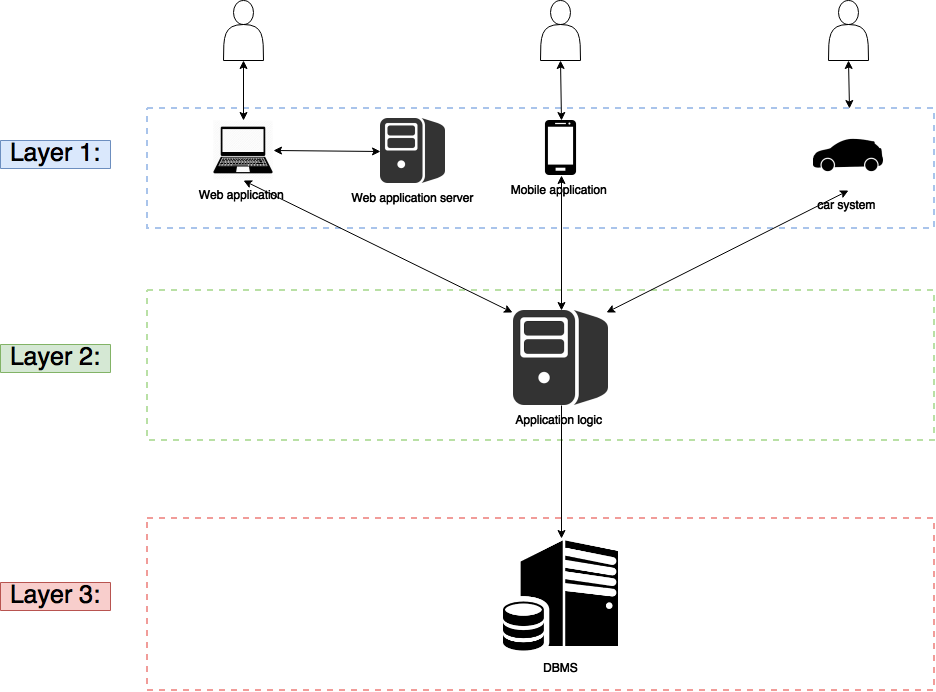
\includegraphics[width=470 pt]{resources/Architectural_structure.png}
\caption{\label{fig:layer}Layers architecture}
\end{figure}

\newpage

\subsection{High level components and their interaction}
In the first level we find two components, the client and the car system. The client is composed of a web application and a mobile application.The web application has to interact with a dedicated server in order to work properly, it should be implemented in java script and HTML and it should have its standalone logic, making to the server only the request for getting data about cars and the map, the request of starting a reservation and the requests of updating the account information. The mobile application should have his standalone logic as well and it will make to the server the same requests as the web application. The car system will be a java application accessible from the car display, through which the user can insert the pin, report damages and end the rent.The request will be send to the server. 
At the second level there is the server,which should be written in php and should have an event driven architecture because it should handle multiple requests at the same time asynchronously. The server interacts with the client by sending notifications about the payments and requesting periodically the position. The server interacts with the car requiring lock/unlock doors and enable engine.The server also requires information such as the position, the remaining charge, the number of passengers and if the car is plugged or not to a charging station.  
At the third level we find the DBMS server that handles a SQL database.
The server interacts with the DBMS with some fetch data request and with some data update requests.

\newpage
\subsection{Component view}
\begin{figure}[hp]
\centering
\includegraphics[width=490 pt]{resources/component.jpg}
\caption{\label{fig:component}Component diagram.}
\end{figure}

\newpage
\subsection{Deployment view}
\begin{figure}[hp]
\centering
\includegraphics[width=470 pt]{resources/deploy.jpg}
\caption{\label{fig:deploy}Deployment diagram.}
\end{figure}

\newpage
\subsection{Runtime view}

\subsubsection*{Reserve a car}
\begin{figure}[hp]
\centering
\includegraphics[width=455 pt]{resources/RunView.jpg}
\caption{\label{fig:reserve}Runtime diagrams for reserve a car.}
\end{figure}

\newpage
\subsubsection*{Rent a car}
\begin{figure}[hp]
\centering
\includegraphics[width=400 pt]{resources/RunView2.jpg}
\caption{\label{fig:startrent}Runtime diagrams for start a rent.}
\end{figure}

\newpage
\subsubsection*{End a rent}
\begin{figure}[hp]
\centering
\includegraphics[width=370 pt]{resources/RunView3.jpg}
\caption{\label{fig:endrent}Runtime diagrams for end a rent.}
\end{figure}


\newpage
\subsection{Component interfaces}
\begin{figure}[hp]
\centering
\includegraphics[width=455 pt]{resources/interface.jpg}
\caption{\label{fig:interface}Component interface diagram.}
\end{figure}


\newpage
\subsection{Selected architectural styles and patterns}
\subparagraph{Overall architecture}\emph{\\}
Our application will be divided into 3 tiers:
\begin{enumerate}
\item  Database handled by a DBMS
\item  Application logic 
\item Thin Client (a simple interface to the application logic layer)
\end{enumerate}
\subparagraph{Design Patterns}\emph{\\}
\textbf{MVC:} The model-view-controller is widely used in our application.The model is represented by the database, the controller is our application logic and the view is the  web app and the mobile app.\\
\textbf{Client-Server} The Client Server Paradigm is used in order to maximize the simplicity of our application.The client is represented by the web application and the mobile application and the server is represented by our application logic and the DBMS

\newpage
\subsection{Other design decisions}
\begin{figure}[hp]
\centering
\includegraphics[width=455 pt]{resources/ER.jpg}
\caption{\label{fig:er}ER diagram.}
\end{figure}


\newpage
\section{Algorithm design
}
Here there is a little view (for example written in Java) of some important algorithm used in the system.
Here below, it is shown how the system indicates a charging station near the destination in order to guarantee a uniform distribution of cars in the city.\\

\begin{lstlisting}
/**
 * Example of some important classes.
 **/

package com.sweng.powerenjoy.routeOptimizer;

import java.util.Math;

public class DistributionOptimizer {

     /** 
     * Calculate the charging station where the client should 
     * release the car to obtain the "money saving" discount.
     *
     * @param destination  The final destination of the client.
     * @throw NotAvailStationException  If there aren't near 
     *                                  stations have a free plug.
     * @return    The position of the recommended charging station.
     */
    static Position RecommendPosDiscount(Position destination) throws NoAvailStationException {
    
        int distance;
        int minCarNumber=Integer.LIMIT_MAX;
        int carNumber;
        ChargingStation rightStation;
        
        for (ChargingStation station : allChargingStations){
            distance=destination.calcDistance(station.getPosition());
            if(distance<MAX_DISTANCE){
                carNumber=station.getNumberCarPlugged();
                if(carNumber<minCarNumber && station.getNumberAvailablePlug()>2){
                    rightStation=station;
                }
            }
        }
        if (rightStation==null)
            throw new NoAvailStationException(destination,MAX_DISTANCE);
        return rightStation.getPosition();
    }
    
}


public class ChargingStation {

    private Position position;
    private int numberPlug;
    private Vector<Car> cars;
    //...
    
    public int getNumberCarPlugged(){
        return numberPlug-this.getNumberAvailablePlug();
    }
    
    int getNumberAvailablePlug(){
    	int n=numberPlug;
    	for(Car car : cars){
        /**
        * For future optimization we can consider the plug 
        * attacched to a reserved car as free.
        * ... && car.getStatus!=Status.RESERVED)
        **/
        	if (car.isPlugged())
            	n--;
        }
        return n;
    }

}

/**
 * One address corresponds to a set of coordinates.
 * There aren't two different position with the same coordinates.
 **/
public class Position {

    private Coordinate coordinate;
    private String addressName;
    private int civicNumber;
    
    public int calcDistance(Position p){
        int x1,x2,y1,y2,d;
        x1=coordinate.getRelativeX();
        y1=coordinate.getRelativeY();
        x2=p.getRelativeX();
        y2=p.getRelativeY();
        d=sqrt( pow(x1-x2,2) + pow(y1-y2,2) );
        return d;
    }
    
}

\end{lstlisting}

\newpage
\section{User interface design}
\subsection{Mockups}
Users can interact with our system through the mobile application, the website and the display located inside the car.

\subsubsection*{View available car information in mobile application} This mockup shows how the information of an available car (charge level and distance from the client) can be displayed in the mobile app. The logged client has the possibility to reserve the car by tapping on the "Reserve" button.
\begin{figure}[hp]
\centering
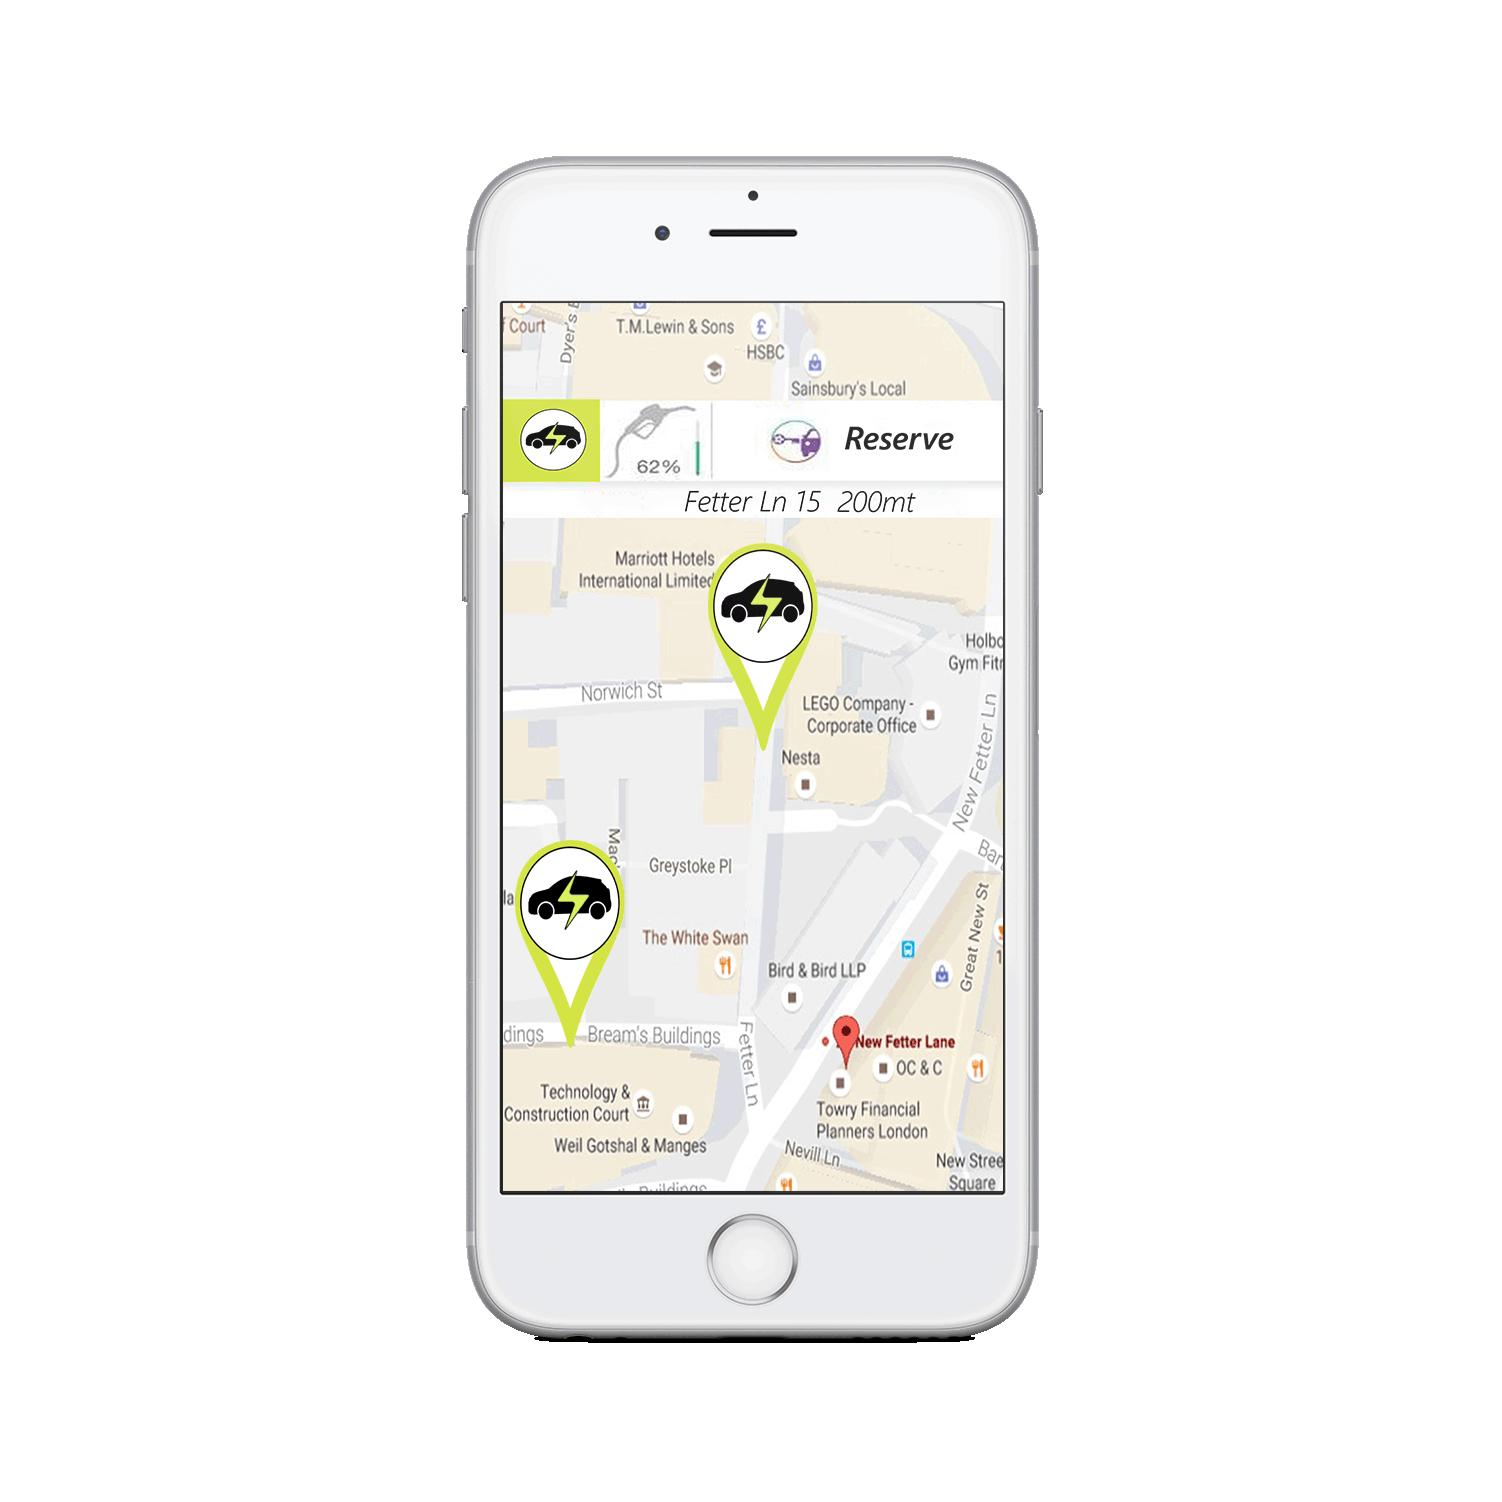
\includegraphics[width=470 pt]{resources/editato.jpg}
\caption{\label{fig:editato}View available car information in mobile application.}
\end{figure}

\newpage

\subsubsection*{View map on the website} This mockup shows the map that a generic user (guest or client) can see on the PowerEnJoy website. On the map are displayed the boundaries of the safe areas in which a client can leave the car and the charging stations with the number of available charging spots. The user can insert an address in order to see the available cars within a certain distance.
\begin{figure}[hp]
\centering
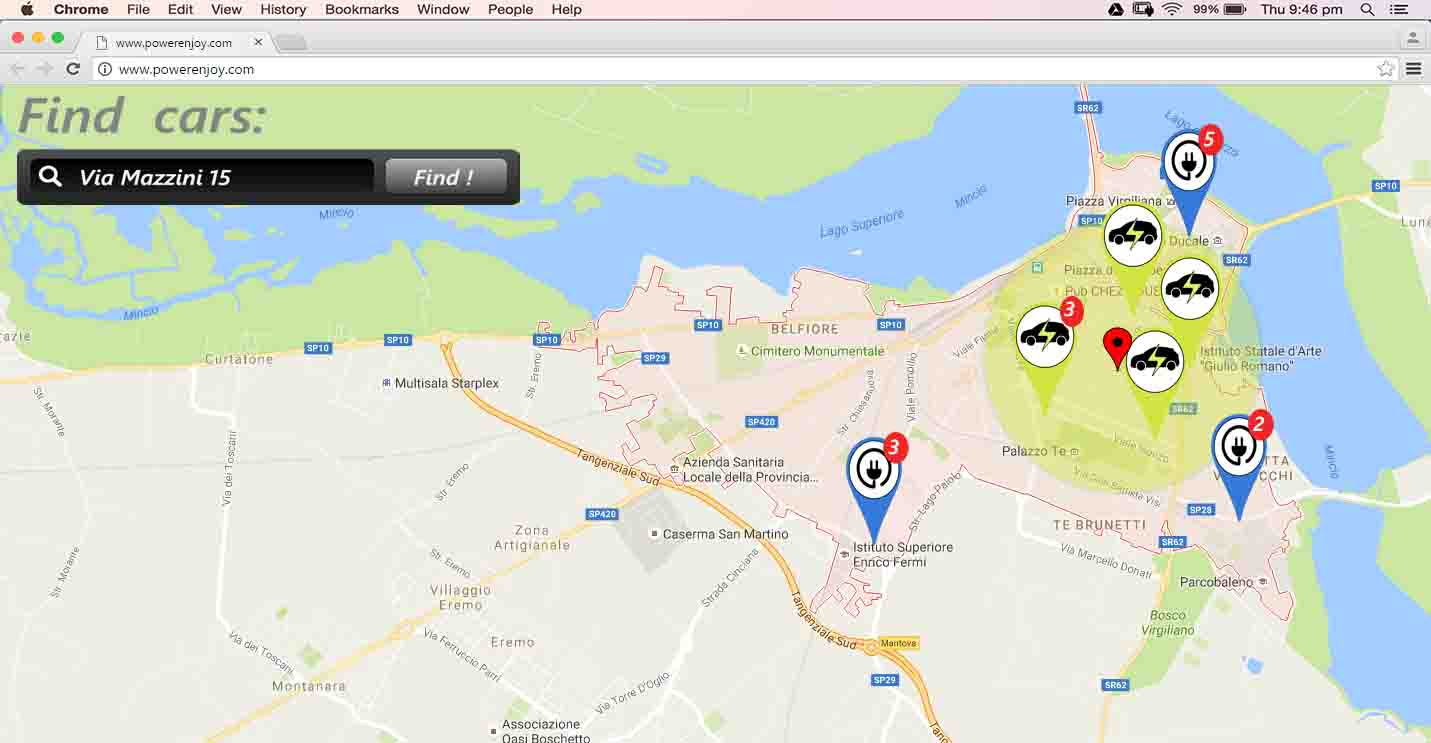
\includegraphics[width=450 pt]{resources/mappa.jpg}
\caption{\label{fig:mappa}View map on the website.}
\end{figure}

\newpage

\subsubsection*{Registration form} The mockup above shows the registration procedure that a guest has to complete in order to become a client and have access to the PowerEnJoy car sharing.

\begin{figure}[hp]
\centering
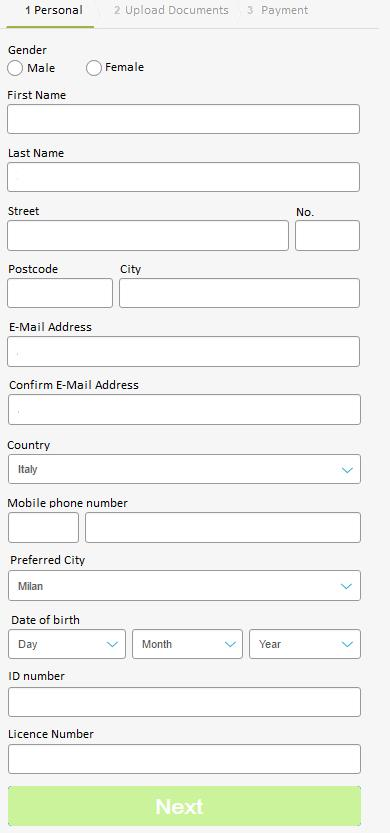
\includegraphics[height=525 pt]{resources/registrazione.jpg}
\caption{\label{fig:reg}Registration form.}
\end{figure}

\newpage

\subsubsection*{Insert pin on the car display} This mockup shows the form in which the client has to insert his pin. After inserting the correct pin the client can start the engine of the car.

\begin{figure}[hp]
\centering
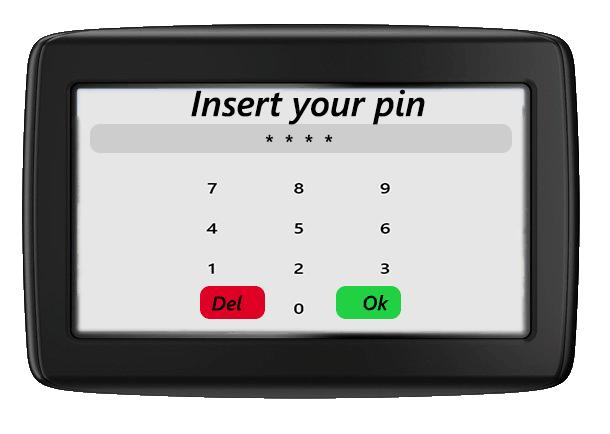
\includegraphics[width=400 pt]{resources/nav68.jpg}
\caption{\label{fig:pin}Insert pin on the car display.}
\end{figure}

\newpage
\subsection{UX Diagrams}
\subsubsection*{UX diagram mobile app}
\begin{figure}[hp]
\centering
\includegraphics[width=400 pt]{resources/UXdiagramApp.jpg}
\caption{\label{fig:uxApp}User Experience diagram app.}
\end{figure}

\newpage
\subsubsection*{UX diagram car}
\begin{figure}[hp]
\centering
\includegraphics[width=400 pt]{resources/UXcar.jpg}
\caption{\label{fig:uxCar}User Experience diagram car.}
\end{figure}

\newpage
\subsection{BCE Diagrams}
\begin{figure}[hp]
\centering
\includegraphics[width=440 pt]{resources/BCE.jpg}
\caption{\label{fig:bce}BCE diagram.}
\end{figure}

\newpage
\section{Requirements traceability}
The design decisions explained in this document have been made in order to satisfy all the goals and requirements presented in the RASD. 
Below, we explain which components of the system have been chosen to satisfy our goals.



\begin{itemize}
\item [G1]A client can register to the system by providing an e-mail, valid payment information and a photo of his driving license.
\begin{itemize}
\item ClientApp
\item UserController
\end{itemize}

\item [G2]A client can log in to system.
\begin{itemize}
\item ClientApp
\item UserController
\end{itemize}

\item [G3]Allows clients to obtain information about available cars(position and remaining charge), safe areas(boundaries) and charging stations (position and available plugs).
\begin{itemize}
\item ClientApp
\item MapController
\end{itemize}

\item [G4]Allows clients to reserve a car that fits most their needs.
\begin{itemize}
\item ClientApp
\item ReservationController
\end{itemize}

\item [G5]A client can start the rent opening a car that has reserved previously when he/she is in the near by.
\begin{itemize}
\item ClientApp
\item RentController
\end{itemize}

\item [G6]During the rent a client can display the amount of money charged.
\begin{itemize}
\item CarRemoteController
\end{itemize}

\item [G7]Guarantee as many available cars as possible encouraging clients to have a virtuous and eco-friendly behavior applying fees and discounts.
\begin{itemize}
\item FareController
\end{itemize}

\item [G8]Allows clients to end the rent and leave the car in any safe area.
\begin{itemize}
\item CarRemoteController
\item CarController
\item RentController
\end{itemize}

\item [G9]Clients can report eventual damages made by users that have driven the car before.
\begin{itemize}
\item CarRemoteController 
\item CarController
\end{itemize}

\item [G10]Clients can set the money saving option.
\begin{itemize}
\item CarRemoteController
\item CarController
\item DistributionOptimizer
\end{itemize}

\end{itemize}

\newpage
\section{Effort spent}
During the whole project the team worked with the following schedule:\\ \emph{\\}
\textbf{Claudio Salvatore Arcidiacono}
\begin{itemize}
\item 29 November : 2 hours
\item 7 December : 15-18 3 hours
\item 8 December : 15-22 5 hours (2hours of pause) 
\item 9 December : 14-18 4 hours\\ 

\textbf{Total hours:} 14 hours.
\end{itemize}


\textbf{Antonio Di Bello}
\begin{itemize}
\item 29 November : 2 hours
\item 5 December : 3 hours
\item 6 December : 3 hours
\item 8 December : 1 hour
\item 9 December : 4 hours
\item 10 December : 2 hours \\

\textbf{Total hours:} 15 hours.
\end{itemize}


\textbf{Denis Dushi}
\begin{itemize}
\item 29 November : 2 hours
\item 6 December : 3 hours
\item 7 December : 3 hours
\item 8 December : 6 hours
\item 10 December : 3 hours
\item 11 December : 1 hours\\

\textbf{Total hours:} 18 hours.
\end{itemize}

\newpage
\section{References}
\subsection{Software and tool used}
The tools we used to create this DD document are:
\begin{itemize}
\item Overleaf (for latex writing in parallel)
\item Photoshop (for mockups)
\item Draw.io (for UML diagrams)
\end{itemize}

\newpage
\listoffigures

\end{document}